    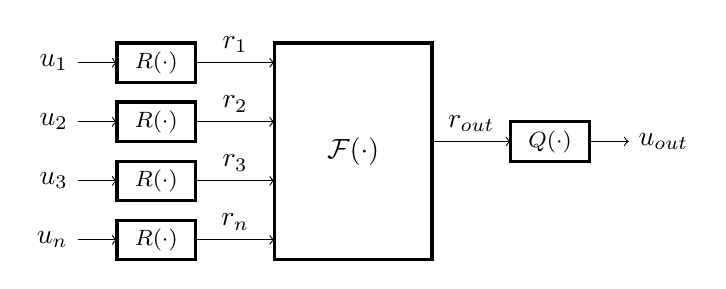
\begin{tikzpicture}[scale=0.5]
    %\draw[help lines, color=gray!30, dashed] (0,0) grid (18,8);
    \draw[black, very thick] (3,1) rectangle (5,2)  node [pos=.5]  {\footnotesize $R(\cdot)$};
    \draw[black, very thick] (3,2.5) rectangle (5,3.5)  node [pos=.5]  {\footnotesize $R(\cdot)$};
    \draw[black, very thick] (3,4) rectangle (5,5)  node [pos=.5]  {\footnotesize $R(\cdot)$};
    \draw[black, very thick] (3,5.5) rectangle (5,6.5)  node [pos=.5]  {\footnotesize $R(\cdot)$};
    \draw [->] (2,1.5) -- (3,1.5);
    \draw [->] (2,3) -- (3,3);
    \draw [->] (2,4.5) -- (3,4.5);
    \draw [->] (2,6) -- (3,6);
    \node [left] at (2,1.5) {$u_{n}$};
    \node [left] at (2,3) {$u_{3}$};
    \node [left] at (2,4.5) {$u_{2}$};
    \node [left] at (2,6) {$u_{1}$};
    \draw [->] (5,1.5) -- (7,1.5);
    \draw [->] (5,3) -- (7,3);
    \draw [->] (5,4.5) -- (7,4.5);
    \draw [->] (5,6) -- (7,6);
    \node [above] at (6,1.5) {$r_{n}$};
    \node [above] at (6,3) {$r_{3}$};
    \node [above] at (6,4.5) {$r_{2}$};
    \node [above] at (6,6) {$r_{1}$};
    \draw[black, very thick] (7,1) rectangle (11,6.5)   node [pos=.5]  { $\mathcal{F}(\cdot)$};
    \draw [->] (11,4) -- (13,4);
    \node [above] at (12,4) {$r_{out}$};
    \draw[black, very thick] (13,3.5) rectangle (15,4.5)  node [pos=.5]  {\footnotesize  $Q(\cdot)$};
    \draw [->] (15,4) -- (16,4);
    \node [right] at (16,4) {$u_{out}$};
    \end{tikzpicture}